Im folgenden Abschnitt wird unsere bewusste Design-Entscheidung der Buttons erklärt. Diese sind ein fundamentales Element jeder Anwendung und müssen richtig gestyled sein. Es ist wichtig, dass Buttons eindeutig erkennbar sind und von anderen Elementen unterschieden werden können.

Beim unserem Kundenmangement Tool wird zwischen zwei Button-Varianten unterschieden:

\begin{itemize}
    \item \textbf{Default Button:}
        \newline
        Dabei handelt es sich um den Default-Button, also die Standard-Version, wobei wir unsere blaue Akzent-Farbe verwendet haben. Grund dafür ist, dass dieser heraussticht und somit eine Aktion symbolisiert. Die Schrift ist weiß, damit der Kontrast zwischen Hintergrund und Schrift hoch ist und damit klar lesbar ist.
        \begin{figure}[h!]
            \centering
            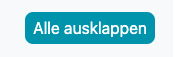
\includegraphics[width=0.3\textwidth]{pics/button-default.png}
            \caption{Default Button Style}
            \label{fig:mesh1}
        \end{figure}
\newpage
    \item \textbf{Outline Button:}
        \newline
        Hierbei handelt es sich um die sogenannte Outline-Variente des Buttons. Dabei hat das Element keine Hintergrundfarbe und wird nur durch einen Rahmen als Button dargestellt. Der unterschied zum Default-Button ist, dass dieser nicht so heraussticht. Diese Variante kann man beispielsweise verwenden, wenn die dadurch ausgelöste Funktion nicht so relevant ist beziehungsweise keine große Änderung verursacht.
        \begin{figure}[h!]
            \centering
            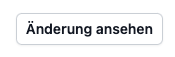
\includegraphics[width=0.3\textwidth]{pics/button-outline.png}
            \caption{Outline Button Style}
            \label{fig:mesh1}
        \end{figure}
\end{itemize}